\documentclass[10pt,twocolumn]{article}
\usepackage[letterpaper,top=0.55in,bottom=0.55in,left=0.6in,right=0.6in,columnsep=0.25in]{geometry}
\usepackage{times}
\usepackage{amsmath,amssymb}
\usepackage{graphicx}
\usepackage{booktabs}
\usepackage[font=normalsize,labelfont=bf,skip=4pt]{caption}
\usepackage[hidelinks]{hyperref}
\usepackage{balance}
\usepackage{titlesec}
\usepackage{multirow}
\usepackage{tikz}
\usetikzlibrary{arrows.meta,positioning,fit,backgrounds,calc,shadows.blur}
% ---- figure palette
\definecolor{cA}{HTML}{1F4E8C}\definecolor{cAbg}{HTML}{DCE8F7}\definecolor{cAin}{HTML}{F5F9FE}
\definecolor{cB}{HTML}{15705A}\definecolor{cBbg}{HTML}{D8EFE6}\definecolor{cBin}{HTML}{F4FBF8}
\definecolor{cC}{HTML}{9A6708}\definecolor{cCbg}{HTML}{FBEED0}\definecolor{cCin}{HTML}{FFFBF0}
\definecolor{cD}{HTML}{9E2F4B}\definecolor{cDbg}{HTML}{FADEE4}\definecolor{cDin}{HTML}{FFF6F8}
\definecolor{slate}{HTML}{2C3A47}
\definecolor{okgr}{HTML}{15705A}
\definecolor{failr}{HTML}{B03A2E}

\pagestyle{empty}
\linespread{0.93}

\titleformat{\section}{\normalsize\bfseries}{\thesection.}{0.5em}{}
\titleformat{\subsection}{\normalsize\bfseries}{\thesubsection.}{0.5em}{}
\titlespacing*{\section}{0pt}{6pt}{3pt}
\titlespacing*{\subsection}{0pt}{5pt}{2pt}
\renewcommand{\thesection}{\arabic{section}}
\renewcommand{\thesubsection}{\thesection.\arabic{subsection}}

\setlength{\parskip}{0pt}
\setlength{\abovedisplayskip}{4pt}
\setlength{\belowdisplayskip}{4pt}
\setlength{\abovecaptionskip}{4pt}
\setlength{\textfloatsep}{8pt}
\newcommand{\tc}{torch.compile}
\newcommand{\fx}{flex\_attention}

\begin{document}

\twocolumn[
\begin{@twocolumnfalse}
\vspace*{2pt}
\begin{center}
{\large\bfseries GraphSynth: Autonomous Optimization of PyTorch Execution Graphs via\\
Search-Guided Compiler Pass \& Triton Kernel Synthesis\par}
\vspace{10pt}
\end{center}
\vspace{2pt}
\end{@twocolumnfalse}
]

\noindent{\normalsize\bfseries Abstract}\vspace{3pt}

\noindent
Static, rule-based lowerings used in MLIR and PyTorch Inductor do not adapt well to
new operator topologies, so memory-bound kernels routinely lose the majority of their
runtime to redundant DRAM traffic, while writing expert Triton or CUDA kernels by hand
takes months of engineering effort per operator. We present GraphSynth, a closed-loop
agentic framework that profiles a PyTorch subgraph, synthesizes a candidate Triton
kernel for it using an LLM, checks the kernel numerically against the PyTorch
reference implementation, and profiles it on real hardware to decide whether to accept
the kernel or iterate.

We evaluate GraphSynth on an NVIDIA A100-SXM4-40GB using ten attention variants that
PyTorch's fused-kernel catalog does not cover. The system produced a verified Triton
kernel for every one of the ten, running 10.83$\times$ faster than eager PyTorch and
3.04$\times$ faster than \tc{}, measured as geometric means over the ten operators. Two
of these kernels are faster than PyTorch's hand-tuned FlashAttention path, because their
masks are sparser than causal attention and a kernel that skips fully masked blocks
therefore does less work. PyTorch's \fx{} remains faster on the eight variants it can
express, by a geometric mean of 1.81$\times$, but it cannot express the remaining two,
which replace the softmax normalization instead of modifying the attention scores.
GraphSynth therefore offers wider coverage and full automation rather than higher peak
performance. As a control, we also ran seven single-tensor operators, where GraphSynth
matches \tc{} exactly (geometric mean 1.00$\times$) and every optimized path converges to
87 to 88\% of peak DRAM bandwidth, showing that the method reports no gain where memory bandwidth
already sets the limit.

\vspace{4pt}
\noindent\textit{Index Terms}: compiler optimization, arithmetic intensity, Triton,
LLM-guided kernel synthesis, GPU roofline analysis.

\section{Introduction}

Deep learning inference performance is bottlenecked by memory bandwidth utilization
rather than raw compute throughput for the majority of operators in modern
architectures. Static compiler backends such as PyTorch Inductor and MLIR-based stacks
rely on rule-based lowering to a fixed catalog of known operators, and any operator or
fusion pattern outside that catalog silently reverts to unfused, sequential execution,
incurring redundant DRAM traffic.

Hand-writing an expert Triton or CUDA kernel to close this gap takes an experienced
engineer weeks to months per operator, and does not scale as new operator topologies
emerge faster than vendor libraries can be hand-tuned. GraphSynth addresses this by
closing the loop between LLM-based kernel synthesis and real hardware feedback. An
autonomous agent profiles a PyTorch subgraph, synthesizes a Triton kernel candidate
from a natural-language operator description, numerically verifies its correctness, and
measures it on hardware, iterating until a verified kernel meets the acceptance
criterion or a budget is exhausted.

Search-based autotuning frameworks such as Ansor and AutoTVM explore tiling and fusion
parameters within a fixed template space, but cannot synthesize new kernel logic.
PyTorch's \fx{} occupies an intermediate position: it admits a user-supplied score
modification into a hand-tuned FlashAttention template, which makes it fast but
restricts it to patterns expressible as a score transform. An LLM-guided approach
instead treats kernel synthesis itself as the search variable.

This paper makes four contributions: (1) a closed-loop PyTorch-to-Triton synthesis
workflow with numerical correctness as a mandatory gate and hardware measurement as the
optimization signal; (2) an arithmetic-intensity criterion that classifies an operator
against the hardware roofline ridge point before any synthesis is attempted; (3) an
evaluation against three baselines (eager PyTorch, \tc{}, and \fx{}), including a
single-tensor control experiment that establishes measurement validity; and (4) the
observation that a synthesized kernel verified at one shape can be silently incorrect
at another.

\section{Overview}

GraphSynth is structured as four sequential stages executed in a closed loop
(Fig.~\ref{fig:loop}): an IR Profiler that classifies operators by arithmetic
intensity, an LLM-driven synthesis stage that writes candidate Triton kernels, a
numerical verifier that rejects incorrect kernels before they reach performance
measurement, and a hardware feedback stage that decides accept-or-iterate. The
separation is intentional: profiling limits the search space to kernels where
optimization is likely to pay off, verification prevents a fast implementation from
being accepted when it changes numerical behavior, and hardware feedback evaluates the
generated program on the target GPU rather than a proxy cost model. A candidate is not
successful merely because it compiles: it must first match the reference and then
satisfy the performance criterion.

\section{Methodology}

\subsection{Platform}

All measurements were taken on a single NVIDIA A100-SXM4-40GB (sm80) on Google Compute
Engine (a2-highgpu-1g), running PyTorch 2.9.1 with CUDA 12.9 and driver
580.178.04. Peak DRAM bandwidth is $BW_{\text{peak}}=1555$~GB/s; peak bf16
tensor-core throughput is 312~TFLOP/s and non-tensor-core fp32 is 19.5~TFLOP/s.

\subsection{Timing protocol and its validation}

An earlier version of this work divided a CUDA-event baseline by an Nsight Compute
kernel latency. The two instruments measure different intervals: events around a single
call absorb host dispatch gaps, while the Nsight counter reports kernel execution only.
A trivial kernel measures 31.7~$\mu$s by the former and ${\approx}2~\mu$s by the latter,
so their ratio inflates any speedup by the dispatch overhead.

\begin{figure}[!t]
\centering
\resizebox{\columnwidth}{!}{%
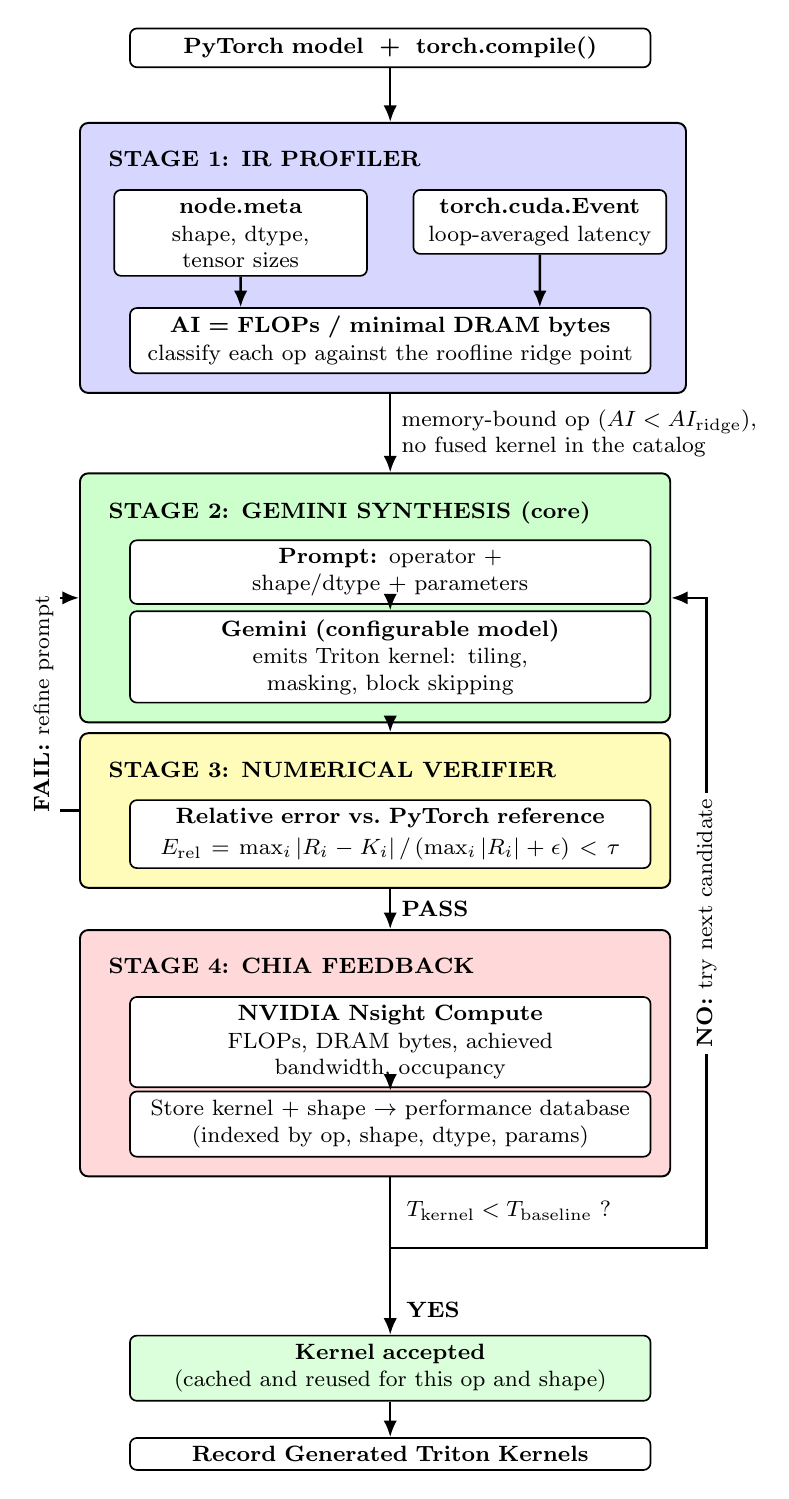
\begin{tikzpicture}[
  x=1mm,y=1mm,
  font=\footnotesize,
  bx/.style ={draw,rounded corners=2.5pt,align=center,inner sep=3pt,line width=0.6pt,fill=white},
  W/.style  ={bx,text width=64mm},
  H/.style  ={bx,text width=30mm},
  pan/.style={draw,rounded corners=3pt,line width=0.7pt,inner sep=2.4mm},
  ar/.style ={-{Latex[length=2.1mm,width=1.7mm]},line width=0.9pt},
  lb/.style ={inner sep=1.4pt},
  st/.style ={font=\footnotesize\bfseries}
]
% ======== top
\node[W,anchor=north] (top) at (0,0) {\bfseries PyTorch model \ + \ torch.compile()};

% ======== stage 1
\node[st,anchor=north west] (t1) at (-37,-14.5) {STAGE 1: IR PROFILER};
\node[H,anchor=north] (meta) at (-19,-20.5)
  {\textbf{node.meta}\\[0.5pt]shape, dtype, tensor sizes};
\node[H,anchor=north] (ev)   at ( 19,-20.5)
  {\textbf{torch.cuda.Event}\\[0.5pt]loop-averaged latency};
\node[W,anchor=north] (s1)   at (0,-35.5)
  {\textbf{AI = FLOPs / minimal DRAM bytes}\\[0.5pt]classify each op against the roofline ridge point};

% ======== stage 2
\node[st,anchor=north west] (t2) at (-37,-59) {STAGE 2: GEMINI SYNTHESIS (core)};
\node[W,anchor=north] (pr) at (0,-65)
  {\textbf{Prompt:} operator + shape/dtype + parameters};
\node[W,anchor=north] (gm) at (0,-74)
  {\textbf{Gemini (configurable model)}\\[0.5pt]emits Triton kernel: tiling, masking, block skipping};

% ======== stage 3
\node[st,anchor=north west] (t3) at (-37,-92) {STAGE 3: NUMERICAL VERIFIER};
\node[W,anchor=north] (vf) at (0,-98)
  {\textbf{Relative error vs.\ PyTorch reference}\\[1.5pt]
   $E_{\text{rel}}=\max_i|R_i-K_i|\,/\,(\max_i|R_i|+\epsilon)<\tau$};

% ======== stage 4
\node[st,anchor=north west] (t4) at (-37,-117) {STAGE 4: CHIA FEEDBACK};
\node[W,anchor=north] (ns) at (0,-123)
  {\textbf{NVIDIA Nsight Compute}\\[0.5pt]FLOPs, DRAM bytes, achieved bandwidth, occupancy};
\node[W,anchor=north] (db) at (0,-135)
  {Store kernel + shape $\rightarrow$ performance database\\[0.5pt](indexed by op, shape, dtype, params)};

% ======== tail
\node[W,anchor=north,fill=green!14] (acc) at (0,-166)
  {\textbf{Kernel accepted}\\[0.5pt](cached and reused for this op and shape)};
\node[W,anchor=north] (rec) at (0,-179)
  {\bfseries Record Generated Triton Kernels};

% ======== stage panels (drawn behind)
\begin{pgfonlayer}{background}
\node[pan,fill=blue!16,  fit=(t1)(meta)(ev)(s1)] (p1) {};
\node[pan,fill=green!20, fit=(t2)(pr)(gm)]       (p2) {};
\node[pan,fill=yellow!28,fit=(t3)(vf)]           (p3) {};
\node[pan,fill=red!15,   fit=(t4)(ns)(db)]       (p4) {};
\end{pgfonlayer}

% ======== forward arrows
\draw[ar] (top.south) -- (top.south |- p1.north);
\draw[ar] (meta.south) -- ([xshift=-19mm]s1.north);
\draw[ar] (ev.south)   -- ([xshift= 19mm]s1.north);
\draw[ar] (s1.south |- p1.south) -- (s1.south |- p2.north)
  node[lb,midway,right=0.8mm,align=left]
  {memory-bound op ($AI<AI_{\text{ridge}}$),\\no fused kernel in the catalog};
\draw[ar] (pr.south) -- (gm.north);
\draw[ar] (gm.south |- p2.south) -- (gm.south |- p3.north);
\draw[ar] (vf.south |- p3.south) -- (vf.south |- p4.north)
  node[lb,midway,right=0.8mm]{\bfseries PASS};
\draw[ar] (ns.south) -- (db.north);
\draw[ar] (db.south |- p4.south) -- (acc.north)
  node[lb,pos=0.21,right=1.4mm,fill=white,inner sep=1.5pt]{$T_{\text{kernel}}<T_{\text{baseline}}$ ?}
  node[lb,pos=0.84,right=1.4mm]{\bfseries YES};
\draw[ar] (acc.south) -- (rec.north);

% ======== feedback loops: start and end on the panel edges, so no line
%          crosses a box or a panel border
\coordinate (fl) at ($(p3.west)+(-4.5,0)$);
\coordinate (nr) at ($(p4.east)+( 4.5,0)$);
% FAIL: verifier panel  ->  synthesis panel   (left side)
\draw[ar] (p3.west) -- (fl) -- (fl |- p2.west) -- (p2.west);
\node[lb,rotate=90,fill=white,inner sep=2.2pt]
  at ($(fl |- p3.west)!0.5!(fl |- p2.west)$)
  {\bfseries FAIL: \mdseries refine prompt};
% NO: too slow  ->  synthesis panel            (right side)
\coordinate (no0) at ($(db.south |- p4.south)+(0,-9)$);
\draw[ar] (no0) -- (no0 -| nr) -- (nr |- p2.east) -- (p2.east);
\node[lb,rotate=90,fill=white,inner sep=2.2pt]
  at ($(nr |- no0)!0.5!(nr |- p2.east)$)
  {\bfseries NO: \mdseries try next candidate};
\end{tikzpicture}}
\caption{GraphSynth autonomous four-stage synthesis loop. Stage~1 classifies an
operator by arithmetic intensity against the device ridge point, Stage~3 gates on
relative error against the PyTorch reference, and Stage~4 accepts only a kernel that is
both correct and faster than the baseline.}
\label{fig:loop}
\end{figure}

All results here use one timing function applied identically to every path: CUDA events
around a \emph{loop} of $n$ invocations, with $n$ adaptive so the timed region spans
${\approx}300$~ms, reporting the median of three repetitions. Bandwidth above 100\% of
peak is physically impossible and is therefore a sufficient falsifier for a timing
method: we calibrate against a device-to-device copy of an $8192{\times}8192$ fp32
tensor, which moves exactly 536.9~MB and performs no arithmetic. It measures
389.6~$\mu$s, i.e.\ 1376~GB/s or 88.6\% of peak. Every bandwidth figure we
report is checked against the 100\% bound; none exceeds it.

\subsection{Correctness gate}

For reference output $R$ and kernel output $K$ we require
\begin{equation}
E_{\text{rel}}=\frac{\max_i|R_i-K_i|}{\max_i|R_i|+\epsilon}<\tau,
\qquad \epsilon=10^{-6},
\end{equation}
with $\tau=10^{-4}$ for fp32 and $3\times10^{-2}$ for bf16, and no NaN or Inf. A
relative criterion is necessary because bf16 attention outputs have magnitude
${\approx}10^{-1}$, for which a fixed absolute tolerance would admit kernels with 20\%
error. Kernels failing the gate are never timed and are reported as failures.

\subsection{Arithmetic intensity and Stage 1 classification}

An ideal fused kernel reads each input once and writes each output once. We take that
minimum traffic $B_{\min}$ as the denominator of bandwidth utilization,
$\eta_{\text{BW}}=B_{\min}/(T\!\cdot\!BW_{\text{peak}})$; because $B_{\min}$ assumes
perfect reuse, every $\eta_{\text{BW}}$ we report is a lower bound. For a single-tensor
operator on an $N{\times}N$ tensor with $b$ bytes per element, $B_{\min}=2N^2b$; for
attention it counts only the query, key, value and output tensors, never the
$S_q{\times}S_{kv}$ score matrix, which a fused kernel keeps on chip.

Arithmetic intensity is $AI=F/B_{\min}$ for $F$ the FLOP count, and an operator is
memory-bound exactly when
\begin{equation}
AI<AI_{\text{ridge}}=FLOP_{\text{peak}}/BW_{\text{peak}},
\end{equation}
which is 200.6~FLOP/byte for bf16 on this device and 12.5 for fp32, giving Stage~1 a
device-derived rather than an arbitrary decision boundary. Attention straddles that
boundary: intensity grows with $S$ during prefill but collapses by three orders of
magnitude in single-token decode, so the same operator family appears on both sides.

\subsection{Baselines}

Each operator is measured along four paths with the same timer: eager
PyTorch; \tc{} (Inductor), which fuses operations and emits Triton, and is
the appropriate baseline for a claim about compiler-generated code; \fx{},
which slots a user-supplied score modification and block mask into a tuned
FlashAttention template; and GraphSynth. We also report fused causal
scaled\_dot\_product\_attention on identically shaped tensors as a hand-tuned
reference, noting it does not implement the semantics under test. \fx{} outputs pass
the same gate. Speedups are latency ratios, aggregated as geometric means.

\section{Results}

\subsection{Control experiment: single-tensor operators}

Table~\ref{tab:single} measures seven single-tensor operators at $8192{\times}8192$ in
fp32, each moving $B_{\min}=536.9$~MB against a DRAM time floor of 345~$\mu$s. All 7/7
were synthesized and verified.

Every path converges to the same ceiling: nineteen of the twenty-one measurements fall
in 391 to 398~$\mu$s, i.e.\ 86.8 to 88.2\% of peak, indistinguishable from the 88.6\% of a
pure device copy. For an operator costing one read and one write this is the hardware
limit. The only two measurements outside that band are the two operators with genuine
headroom, eager softmax at 75.4\% and eager layernorm at 58.4\%, which materialize intermediates for their reductions, are closed identically by
both systems (1.15$\times$ and 1.49$\times$); the five pointwise operators were already
at the ceiling and correctly report 1.00$\times$.

GraphSynth does not outperform Inductor here: 1 of 7 operators, geometric mean
1.00$\times$. We report this as a negative result, and as the expected one, since these
operators lie inside Inductor's fusion coverage and both systems hit the same memory
wall. Its value is that the methodology reports parity where theory demands parity,
which is the precondition for interpreting Table~\ref{tab:attn}.

\begin{table*}[t]
\centering
\caption{Single-tensor operators (control). fp32, $[8192,8192]$; $B_{\min}=536.9$~MB;
DRAM time floor 345~$\mu$s. A pure device copy reaches 88.6\% (389.6~$\mu$s) and is the
practical ceiling. ``compile'' is \tc{} (Inductor). All latencies in $\mu$s, medians of
three repetitions.}
\label{tab:single}
\setlength{\tabcolsep}{3pt}
\begin{tabular}{lrrrrcrrrr}
\toprule
& \multicolumn{2}{c}{Eager PyTorch} & \multicolumn{2}{c}{compile}
& compile & \multicolumn{2}{c}{GraphSynth} & \multicolumn{2}{c}{GraphSynth vs.} \\
\cmidrule(lr){2-3}\cmidrule(lr){4-5}\cmidrule(lr){7-8}\cmidrule(lr){9-10}
Operator & $T$ & $\eta_{\text{BW}}$ & $T$ & $\eta_{\text{BW}}$ & $\times$
& $T$ & $\eta_{\text{BW}}$ & eager & compile \\
\midrule
relu        & 393 & 87.9\% & 392 & 88.2\% & 1.00$\times$ & 394 & 87.7\% & 1.00$\times$ & 0.99$\times$ \\
leaky\_relu & 393 & 87.9\% & 393 & 87.7\% & 1.00$\times$ & 396 & 87.2\% & 0.99$\times$ & 0.99$\times$ \\
sigmoid     & 393 & 87.8\% & 394 & 87.7\% & 1.00$\times$ & 393 & 87.8\% & 1.00$\times$ & 1.00$\times$ \\
silu        & 393 & 87.8\% & 394 & 87.7\% & 1.00$\times$ & 393 & 87.9\% & 1.00$\times$ & 1.00$\times$ \\
gelu        & 393 & 87.9\% & 395 & 87.4\% & 0.99$\times$ & 392 & 88.0\% & 1.00$\times$ & 1.01$\times$ \\
softmax     & 458 & 75.4\% & 397 & 87.0\% & 1.15$\times$ & 397 & 86.9\% & 1.15$\times$ & 1.00$\times$ \\
layernorm   & 591 & 58.4\% & 396 & 87.2\% & 1.49$\times$ & 398 & 86.8\% & 1.49$\times$ & 0.99$\times$ \\
\midrule
geometric mean & & & & & 1.08$\times$ & & & 1.08$\times$ & 1.00$\times$ \\
\bottomrule
\end{tabular}
\end{table*}

\begin{table*}[t]
\centering
\caption{Attention variants outside PyTorch's fused-kernel catalog. bf16, $B{=}2$,
$H{=}32$, $S{=}2048$, $D{=}128$. Latencies in $\mu$s. ``compile'' is \tc{} and ``flex''
is \fx{}; ``model'' gives the faster of the two LLM backends (2.5${=}$gemini-2.5-pro,
3.1${=}$gemini-3.1-pro-preview). All columns are computed from a single measurement run. Fused causal
FlashAttention on identical tensors: 457~$\mu$s. ``n/a'' marks operators flex cannot express, as they replace softmax
normalization rather than modifying scores. Sorted by speedup over eager.}
\label{tab:attn}
\setlength{\tabcolsep}{3pt}
\begin{tabular}{lrrrrcrrr}
\toprule
& \multicolumn{3}{c}{Baseline latency} & \multicolumn{2}{c}{GraphSynth}
& \multicolumn{3}{c}{GraphSynth speedup vs.} \\
\cmidrule(lr){2-4}\cmidrule(lr){5-6}\cmidrule(lr){7-9}
Operator & eager & compile & flex & $T$ & model & eager & compile & flex \\
\midrule
block-diagonal mask   &  8251 & 2580 & 261 &  289 & 3.1 & 28.51$\times$ & 8.91$\times$ & 0.90$\times$ \\
sliding-window mask   &  8330 & 2582 & 226 &  433 & 3.1 & 19.24$\times$ & 5.96$\times$ & 0.52$\times$ \\
ReLU attention        &  8534 & 1994 & n/a &  473 & 2.5 & 18.05$\times$ & 4.22$\times$ & n/a          \\
ALiBi bias            & 11076 & 2623 & 641 &  841 & 3.1 & 13.16$\times$ & 3.12$\times$ & 0.76$\times$ \\
local (banded) mask   &  8390 & 2640 & 402 &  662 & 3.1 & 12.68$\times$ & 3.99$\times$ & 0.61$\times$ \\
logit soft-capping    & 10645 & 3133 & 847 &  901 & 3.1 & 11.81$\times$ & 3.48$\times$ & 0.94$\times$ \\
sigmoid attention     &  8534 & 1991 & n/a & 1073 & 2.5 &  7.95$\times$ & 1.86$\times$ & n/a          \\
prefix-LM mask        &  8335 & 2579 & 557 & 1390 & 3.1 &  6.00$\times$ & 1.86$\times$ & 0.40$\times$ \\
per-head temperature  &  9521 & 2637 & 614 & 1864 & 2.5 &  5.11$\times$ & 1.41$\times$ & 0.33$\times$ \\
dilated mask          &  8442 & 2585 & 571 & 1817 & 3.1 &  4.65$\times$ & 1.42$\times$ & 0.31$\times$ \\
\midrule
geometric mean & & & & & & 10.83$\times$ & 3.04$\times$ & 0.55$\times$ \\
\bottomrule
\end{tabular}
\end{table*}

\subsection{Attention variants outside the fused catalog}

PyTorch's fused attention path supports three configurations: unmasked, causal, and
grouped-query. Table~\ref{tab:attn} measures ten variants outside it. All 10/10
produced a numerically verified kernel.

GraphSynth beats eager PyTorch and \tc{} on every operator, by
4.65$\times$ to 28.51$\times$ (geometric mean 10.83$\times$) and 1.41$\times$ to
8.91$\times$ (geometric mean 3.04$\times$) respectively. Inductor is not a weak
baseline: it delivers 3.18$\times$ to 4.29$\times$ over eager on every operator
(geometric mean 3.56$\times$), fusing the score computation and removing intermediate
materialization, so the residual gap is not an artifact of an unoptimized comparison.

The gap is structural rather than incidental. Inductor fuses the operations the user
wrote but does not change the algorithm: a dense attn\_mask argument still
forces computation of all $S^2$ scores followed by masking. The synthesized kernels
instead compute the mask predicate from tile indices and bound the key/value loop so
that fully masked blocks are never visited. The effect is largest where the mask is
sparsest: block-diagonal masking (four 512-token documents) reaches 289~$\mu$s and
sliding-window masking (width 256, ${\approx}12\%$ density) 433~$\mu$s. Both are
\emph{faster than FlashAttention itself} (0.63$\times$ and 0.95$\times$ of the
457~$\mu$s fused causal reference), which is not a contradiction: both masks are
strictly sparser than causal, so a block-skipping kernel does strictly less work.

\fx{} is faster than GraphSynth wherever it applies, and we report it. On the
eight operators it can express it wins all eight (geometric mean ratio 0.55$\times$,
i.e.\ \fx{} is 1.81$\times$ faster), narrowly on soft-capping (0.94$\times$) and
block-diagonal masking (0.90$\times$) and widely on dilated masking (0.31$\times$).
This is the expected consequence of template reuse: \fx{} inherits an expert-tuned
FlashAttention schedule, whereas GraphSynth must rediscover that tuning. \fx{} cannot,
however, express two of the ten: its abstraction modifies \emph{scores} but fixes
softmax as the normalization, so sigmoid and ReLU attention lie outside it whatever
modification is supplied. The template compiler is faster inside its expressible set;
the synthesizer has a larger expressible set.

\subsection{Sparsity is specified but not executed}

Across eleven mask patterns characterized in Stage~1 (sliding-window, dilated, local,
block-sparse, block-diagonal, prefix-LM, Longformer, BigBird and others), measured
latency varied by under 6\% (1707 to 1802~$\mu$s at $S{=}2048$) while the underlying
densities differ by more than 2$\times$. All eleven dispatched to the same cuDNN masked
path, and a sliding-window mask covering ${\approx}12\%$ of the score matrix ran
3.27$\times$ \emph{slower} than full causal attention. Mechanisms designed to reduce
attention from $O(S^2)$ to $O(S\!\cdot\!w)$ therefore keep their asymptotic claim in the
model definition while executing densely on this stack.

\subsection{Synthesis convergence}

Each operator was allowed at most three iterations, with compilation errors,
verification failures and measured latency appended to the prompt on each retry.
gemini-3.1-pro-preview accepted 10/10, all on the first iteration, and produced
the faster kernel on 7 of 10; gemini-2.5-pro accepted 9/10 at a mean of 1.4
iterations, failing to converge on dilated masking within the budget.

One reported failure was a specification defect: sigmoid attention initially failed for
both backends with an identical relative error of ${\approx}0.8$, traced to our reference
applying the mask before the sigmoid rather than after. An error identical across models
and iterations is diagnostic of the specification, not the generated code.

The feedback loop is visible in the released traces. On logit soft-capping,
iteration~1 emitted tl.math.tanh, absent from this Triton version; iteration~2,
given that error, used the removed tl.dot(trans\_b=True); iteration~3, given
both, compiled and verified. No generated kernel was edited by hand.

\subsection{Shape generalization and a silent-correctness hazard}

Kernels were synthesized at $S{=}2048$ only. Re-verifying each accepted kernel at
$S\in\{1024,2048,4096\}$ (Table~\ref{tab:shape}) shows that for all ten operators at
least one backend produced a kernel correct at all three lengths, and that speedups are
stable or improve with $S$. The extreme case is block-diagonal masking at $S{=}4096$,
at 562~$\mu$s against 34183~$\mu$s eager (60.88$\times$). The advantage is
therefore not an artifact of the synthesis shape. The backends differ sharply in shape
generality despite the same prompt: four gemini-2.5-pro kernels hardcoded the
synthesis shape and raise AssertionError at any $S\neq2048$.

One failure mode deserves emphasis. The gemini-3.1-pro-preview kernel for
prefix-LM masking passes the gate at $S{=}1024$ ($E_{\text{rel}}{=}1.5\times10^{-2}$)
and $S{=}2048$ ($1.2\times10^{-2}$), but at $S{=}4096$ returns a 23\% relative error.
It does not raise, does not return the wrong shape, and does not produce NaN: it
silently computes the wrong answer. An acceptance gate evaluated at one shape therefore
does not certify a kernel at another: a deployed system must re-verify per shape, or
restrict each cached kernel to its verified configuration. A second pathological case:
one ReLU-attention kernel verifies at all three lengths while running at
${\approx}0.20\times$ of eager at every one, so a gate on correctness alone admits
performance regressions.

\begin{table}[t]
\centering
\caption{Shape generalization. Kernels were synthesized at $S{=}2048$ only.
``Correct'' counts kernels passing the full correctness gate at that $S$; geometric
means are over that backend's correct kernels.}
\label{tab:shape}
\setlength{\tabcolsep}{3.5pt}
\begin{tabular}{llcc}
\toprule
Backend & $S$ & Correct & Geo.\ mean \\
\midrule
\multirow{3}{*}{2.5-pro}
 & 1024 & 5/9   & 5.71$\times$ \\
 & 2048 & 9/9   & 6.77$\times$ \\
 & 4096 & 5/9   & 7.42$\times$ \\
\midrule
\multirow{3}{*}{3.1-pro-preview}
 & 1024 & 10/10 & 4.79$\times$ \\
 & 2048 & 10/10 & 6.60$\times$ \\
 & 4096 & 9/10  & 8.85$\times$ \\
\bottomrule
\end{tabular}
\end{table}

\section{Limitations}

\fx{} is faster where it applies. On the eight of ten operators expressible as
a score modification plus block mask it wins all eight (geometric mean 1.81$\times$). We
make no claim of performance superiority over it; our claim is coverage, 10/10 versus
8/10, and interface, since GraphSynth consumes a natural-language operator description
whereas \fx{} requires the pattern hand-written in a prescribed form plus a separately
constructed block mask. Inside PyTorch's existing fusion coverage we claim nothing:
GraphSynth beats \tc{} on 1 of 7 single-tensor operators.

On measurement and scope, everything reported here was re-measured with the single
validated timer of Sec.~3.2, superseding the mixed-instrument figures of our earlier
report. All results come from one A100-SXM4-40GB, forward pass only, with a single
synthesis trial per cell, so we report no variance. Synthesized kernels are also not
reliably shape-general, as Sec.~4.5 shows.

\section{Related Work}

cuDNN and cuBLAS provide hand-tuned kernels for a fixed operator set with no capability
for novel topologies. Ansor and AutoTVM search tiling parameters within existing
templates but cannot synthesize new kernel logic. MLIR and Triton provide the compiler
infrastructure GraphSynth builds on, and PyTorch~2 the graph-compilation substrate.
PyTorch's \fx{} is the closest prior system, compiling a user-supplied score
modification into a tuned FlashAttention template; our measurements show it is faster
than GraphSynth wherever the pattern is expressible in that form. GraphSynth's novelty
is combining synthesis of new kernel logic, which is not bound to a template and
therefore covers replaced normalizations that \fx{} cannot express, with hardware-measured
refinement and numerical verification as a mandatory gate.

\section{Conclusion}

GraphSynth closes the loop between LLM kernel synthesis and hardware measurement, with
numerical verification as a mandatory gate. On ten attention variants outside PyTorch's
fused-kernel catalog it produced verified Triton kernels for all ten, improving on eager
PyTorch by a geometric mean of 10.83$\times$ and on \tc{} by 3.04$\times$, with two
kernels faster than PyTorch's hand-tuned FlashAttention path. A single-tensor control
experiment reports parity with \tc{} at 87 to 88\% of peak bandwidth, confirming the
methodology does not manufacture speedups where the memory wall forecloses them. Where
\fx{} applies it is 1.81$\times$ faster; GraphSynth's contribution is the larger
expressible set and the absence of any hand-written kernel specification. Finally, a
kernel verified at one sequence length can be silently incorrect at another, so
per-shape re-verification is a requirement for any system deploying LLM-generated
kernels.

\par\vspace{8pt}
\noindent{\normalsize\bfseries Acknowledgment of AI Assistance}\vspace{3pt}

\noindent
Portions of this manuscript's drafting, code implementation, debugging, and figure
preparation were assisted by Claude (Anthropic). All experimental results, design
decisions, and conclusions were reviewed and verified by the human authors, who take full
responsibility for the entire content, tone, and quality of this paper.

\balance
\begin{thebibliography}{5}
\setlength{\itemsep}{0pt}\setlength{\parskip}{0pt}
\bibitem{mlir} C.~Lattner \textit{et al.}, ``MLIR: Scaling Compiler Infrastructure for Domain Specific Computation,'' in \textit{Proc. IEEE/ACM CGO}, 2021.
\bibitem{triton} P.~Tillet, H.~T. Kung, and D.~Cox, ``Triton: An Intermediate Language and Compiler for Tile-Based Neural Network Programs,'' in \textit{Proc. ACM MAPL}, 2019.
\bibitem{chia} A.~Cui \textit{et al.}, ``CHIA: Agentic Approaches to Architecture,'' MICRO 2026, arXiv:2606.27350.
\bibitem{ansor} L.~Zheng \textit{et al.}, ``Ansor: Generating High-Performance Tensor Programs for Deep Learning,'' in \textit{Proc. USENIX OSDI}, 2020.
\bibitem{pt2} J.~Ansel \textit{et al.}, ``PyTorch 2: Faster Machine Learning Through Dynamic Python Bytecode Transformation and Graph Compilation,'' in \textit{Proc. ACM ASPLOS}, 2024.
\end{thebibliography}

\end{document}
